% Triton kernel memory savings bar chart
% Compile: pdflatex kernel_memsave.tex
% Inline:  % Triton kernel memory savings bar chart
% Compile: pdflatex kernel_memsave.tex
% Inline:  % Triton kernel memory savings bar chart
% Compile: pdflatex kernel_memsave.tex
% Inline:  % Triton kernel memory savings bar chart
% Compile: pdflatex kernel_memsave.tex
% Inline:  \input{figures/kernel_memsave.tex}
%
% 数据来源:
%   profile_v2_h800.md   (forward-only)   — Mem Save 列
%   profile_bwd_h800.md  (forward+backward) — Mem Save 列
% 测试硬件: NVIDIA H800 PCIe
% 测试形状: B=64, T=3072, d_model=448, d_ff=1216, h=7, V=256, bf16
%
% 设计要点:
%   - 线性 y 轴 (0%-90%): 数据范围 0%-80%, 无需 log
%   - x 轴顺序与 kernel_speedup.tex 完全一致: 方便交叉对照"加速 vs 显存"
%   - 41.1% 均值参考线: 用 extra y ticks + grid style 实现 (避免 axis cs +
%     symbolic coords 组合在部分 pgfplots 版本下的解析失败)
\documentclass[tikz,border=10pt]{standalone}
\usepackage{pgfplots}
\usepackage{amsmath}
\pgfplotsset{compat=1.17}

\begin{document}
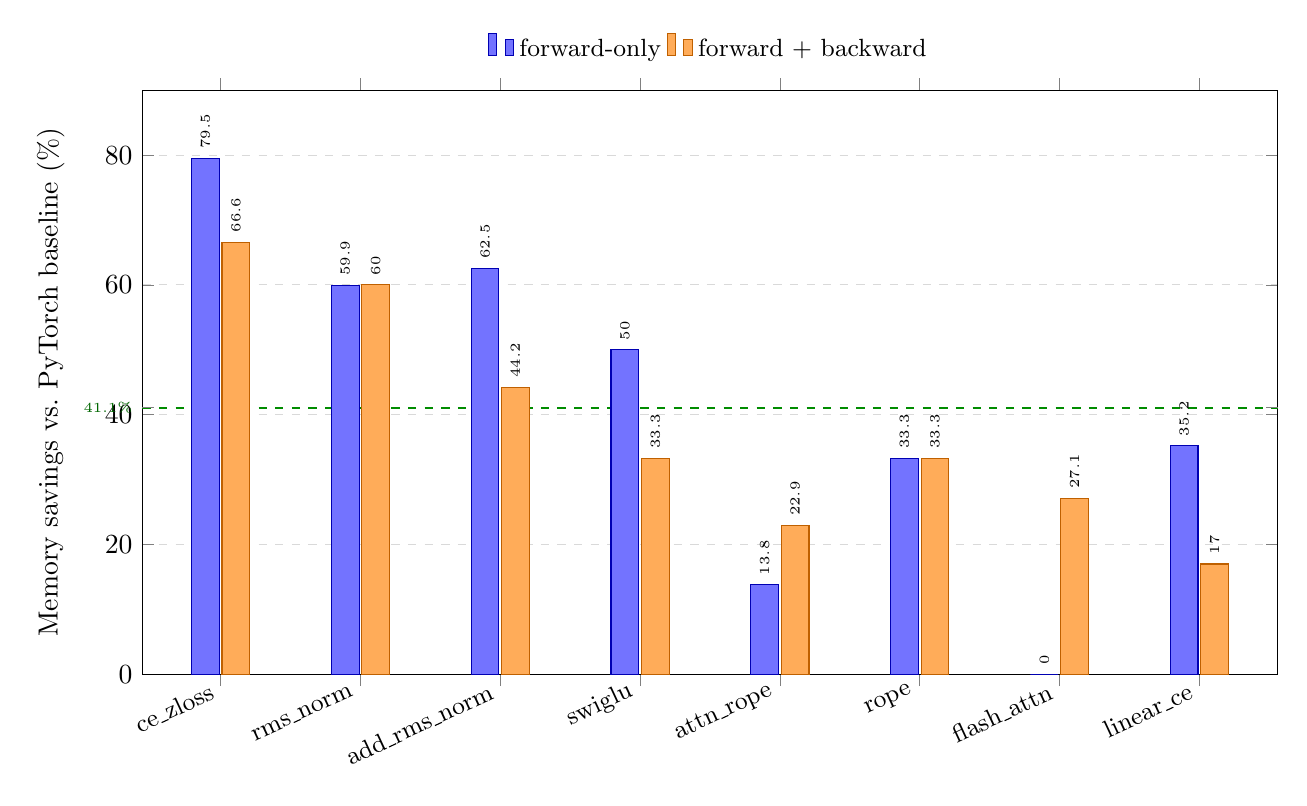
\begin{tikzpicture}
\begin{axis}[
    ybar=1pt,
    bar width=10pt,
    width=16cm,
    height=9cm,
    ymin=0,
    ymax=90,
    ylabel={Memory savings vs.\ PyTorch baseline (\%)},
    symbolic x coords={
        ce\_zloss,
        rms\_norm,
        add\_rms\_norm,
        swiglu,
        attn\_rope,
        rope,
        flash\_attn,
        linear\_ce
    },
    xtick=data,
    x tick label style={rotate=25, anchor=east, font=\small},
    enlarge x limits=0.08,
    legend style={
        at={(0.5,1.03)},
        anchor=south,
        legend columns=2,
        font=\small,
        draw=none
    },
    ymajorgrids=true,
    grid style={dashed, gray!30},
    % 41.1% 均值参考线 (7 个生效算子 fwd+bwd 平均)
    extra y ticks={41.1},
    extra y tick labels={41.1\%},
    extra y tick style={
        grid=major,
        grid style={dashed, green!55!black, line width=0.7pt},
        tick label style={green!40!black, font=\tiny}
    },
    nodes near coords,
    every node near coord/.append style={
        font=\tiny,
        rotate=90,
        anchor=west,
        /pgf/number format/.cd, fixed, precision=1
    },
]

% forward-only memory savings (蓝色) — 数据来自 profile_v2_h800.md
\addplot[fill=blue!55, draw=blue!70!black] coordinates {
    (ce\_zloss,      79.5)
    (rms\_norm,      59.9)
    (add\_rms\_norm, 62.5)
    (swiglu,         50.0)
    (attn\_rope,     13.8)
    (rope,           33.3)
    (flash\_attn,     0.0)
    (linear\_ce,     35.2)
};
\addlegendentry{forward-only}

% forward + backward memory savings (橙色) — 数据来自 profile_bwd_h800.md
\addplot[fill=orange!65, draw=orange!75!black] coordinates {
    (ce\_zloss,      66.6)
    (rms\_norm,      60.0)
    (add\_rms\_norm, 44.2)
    (swiglu,         33.3)
    (attn\_rope,     22.9)
    (rope,           33.3)
    (flash\_attn,    27.1)
    (linear\_ce,     17.0)
};
\addlegendentry{forward + backward}

\end{axis}
\end{tikzpicture}
\end{document}

%
% 数据来源:
%   profile_v2_h800.md   (forward-only)   — Mem Save 列
%   profile_bwd_h800.md  (forward+backward) — Mem Save 列
% 测试硬件: NVIDIA H800 PCIe
% 测试形状: B=64, T=3072, d_model=448, d_ff=1216, h=7, V=256, bf16
%
% 设计要点:
%   - 线性 y 轴 (0%-90%): 数据范围 0%-80%, 无需 log
%   - x 轴顺序与 kernel_speedup.tex 完全一致: 方便交叉对照"加速 vs 显存"
%   - 41.1% 均值参考线: 用 extra y ticks + grid style 实现 (避免 axis cs +
%     symbolic coords 组合在部分 pgfplots 版本下的解析失败)
\documentclass[tikz,border=10pt]{standalone}
\usepackage{pgfplots}
\usepackage{amsmath}
\pgfplotsset{compat=1.17}

\begin{document}
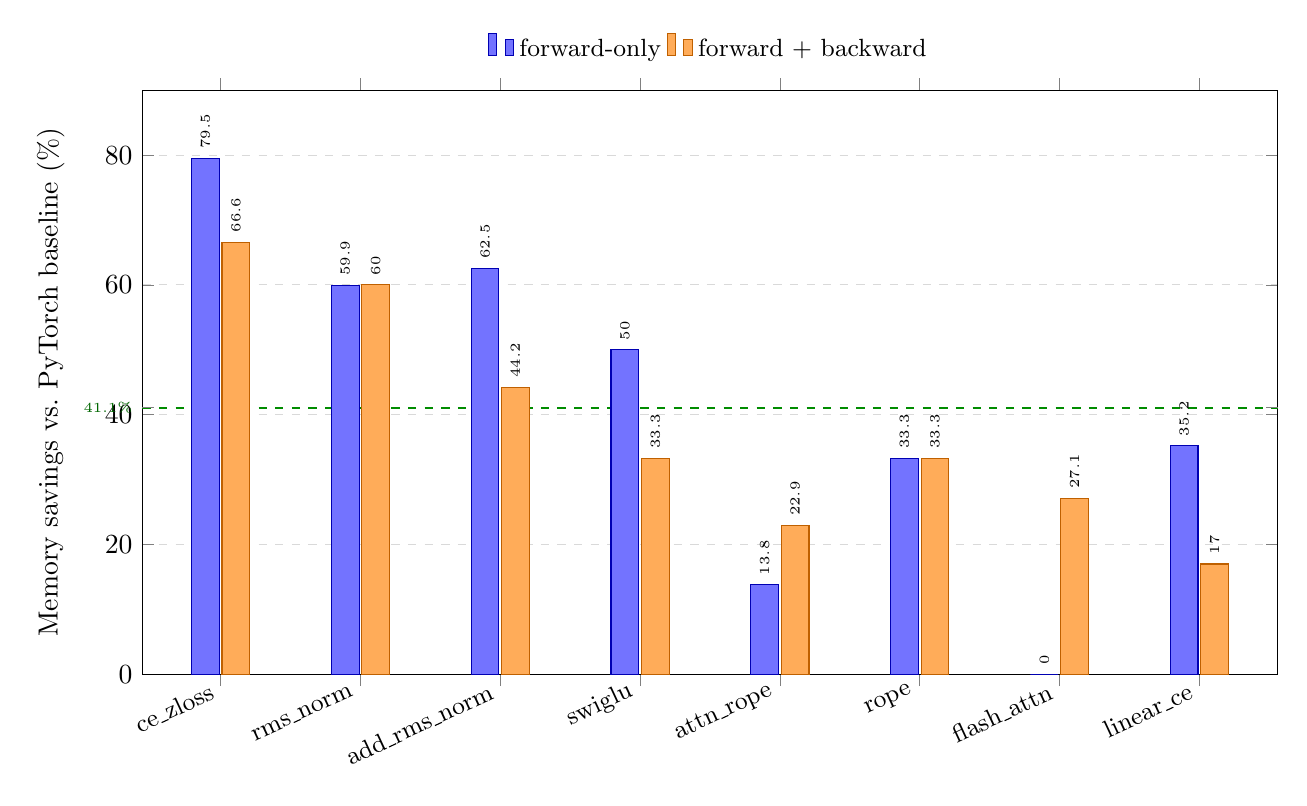
\begin{tikzpicture}
\begin{axis}[
    ybar=1pt,
    bar width=10pt,
    width=16cm,
    height=9cm,
    ymin=0,
    ymax=90,
    ylabel={Memory savings vs.\ PyTorch baseline (\%)},
    symbolic x coords={
        ce\_zloss,
        rms\_norm,
        add\_rms\_norm,
        swiglu,
        attn\_rope,
        rope,
        flash\_attn,
        linear\_ce
    },
    xtick=data,
    x tick label style={rotate=25, anchor=east, font=\small},
    enlarge x limits=0.08,
    legend style={
        at={(0.5,1.03)},
        anchor=south,
        legend columns=2,
        font=\small,
        draw=none
    },
    ymajorgrids=true,
    grid style={dashed, gray!30},
    % 41.1% 均值参考线 (7 个生效算子 fwd+bwd 平均)
    extra y ticks={41.1},
    extra y tick labels={41.1\%},
    extra y tick style={
        grid=major,
        grid style={dashed, green!55!black, line width=0.7pt},
        tick label style={green!40!black, font=\tiny}
    },
    nodes near coords,
    every node near coord/.append style={
        font=\tiny,
        rotate=90,
        anchor=west,
        /pgf/number format/.cd, fixed, precision=1
    },
]

% forward-only memory savings (蓝色) — 数据来自 profile_v2_h800.md
\addplot[fill=blue!55, draw=blue!70!black] coordinates {
    (ce\_zloss,      79.5)
    (rms\_norm,      59.9)
    (add\_rms\_norm, 62.5)
    (swiglu,         50.0)
    (attn\_rope,     13.8)
    (rope,           33.3)
    (flash\_attn,     0.0)
    (linear\_ce,     35.2)
};
\addlegendentry{forward-only}

% forward + backward memory savings (橙色) — 数据来自 profile_bwd_h800.md
\addplot[fill=orange!65, draw=orange!75!black] coordinates {
    (ce\_zloss,      66.6)
    (rms\_norm,      60.0)
    (add\_rms\_norm, 44.2)
    (swiglu,         33.3)
    (attn\_rope,     22.9)
    (rope,           33.3)
    (flash\_attn,    27.1)
    (linear\_ce,     17.0)
};
\addlegendentry{forward + backward}

\end{axis}
\end{tikzpicture}
\end{document}

%
% 数据来源:
%   profile_v2_h800.md   (forward-only)   — Mem Save 列
%   profile_bwd_h800.md  (forward+backward) — Mem Save 列
% 测试硬件: NVIDIA H800 PCIe
% 测试形状: B=64, T=3072, d_model=448, d_ff=1216, h=7, V=256, bf16
%
% 设计要点:
%   - 线性 y 轴 (0%-90%): 数据范围 0%-80%, 无需 log
%   - x 轴顺序与 kernel_speedup.tex 完全一致: 方便交叉对照"加速 vs 显存"
%   - 41.1% 均值参考线: 用 extra y ticks + grid style 实现 (避免 axis cs +
%     symbolic coords 组合在部分 pgfplots 版本下的解析失败)
\documentclass[tikz,border=10pt]{standalone}
\usepackage{pgfplots}
\usepackage{amsmath}
\pgfplotsset{compat=1.17}

\begin{document}
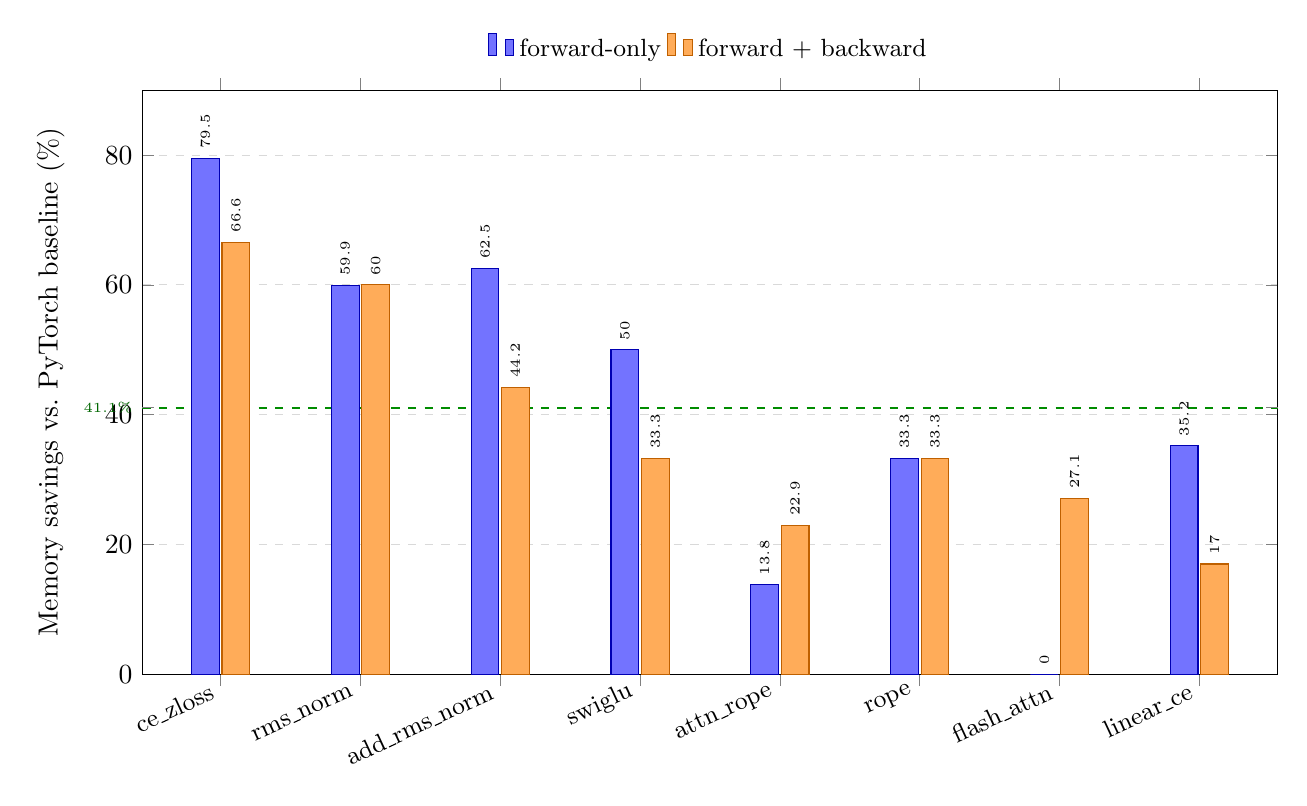
\begin{tikzpicture}
\begin{axis}[
    ybar=1pt,
    bar width=10pt,
    width=16cm,
    height=9cm,
    ymin=0,
    ymax=90,
    ylabel={Memory savings vs.\ PyTorch baseline (\%)},
    symbolic x coords={
        ce\_zloss,
        rms\_norm,
        add\_rms\_norm,
        swiglu,
        attn\_rope,
        rope,
        flash\_attn,
        linear\_ce
    },
    xtick=data,
    x tick label style={rotate=25, anchor=east, font=\small},
    enlarge x limits=0.08,
    legend style={
        at={(0.5,1.03)},
        anchor=south,
        legend columns=2,
        font=\small,
        draw=none
    },
    ymajorgrids=true,
    grid style={dashed, gray!30},
    % 41.1% 均值参考线 (7 个生效算子 fwd+bwd 平均)
    extra y ticks={41.1},
    extra y tick labels={41.1\%},
    extra y tick style={
        grid=major,
        grid style={dashed, green!55!black, line width=0.7pt},
        tick label style={green!40!black, font=\tiny}
    },
    nodes near coords,
    every node near coord/.append style={
        font=\tiny,
        rotate=90,
        anchor=west,
        /pgf/number format/.cd, fixed, precision=1
    },
]

% forward-only memory savings (蓝色) — 数据来自 profile_v2_h800.md
\addplot[fill=blue!55, draw=blue!70!black] coordinates {
    (ce\_zloss,      79.5)
    (rms\_norm,      59.9)
    (add\_rms\_norm, 62.5)
    (swiglu,         50.0)
    (attn\_rope,     13.8)
    (rope,           33.3)
    (flash\_attn,     0.0)
    (linear\_ce,     35.2)
};
\addlegendentry{forward-only}

% forward + backward memory savings (橙色) — 数据来自 profile_bwd_h800.md
\addplot[fill=orange!65, draw=orange!75!black] coordinates {
    (ce\_zloss,      66.6)
    (rms\_norm,      60.0)
    (add\_rms\_norm, 44.2)
    (swiglu,         33.3)
    (attn\_rope,     22.9)
    (rope,           33.3)
    (flash\_attn,    27.1)
    (linear\_ce,     17.0)
};
\addlegendentry{forward + backward}

\end{axis}
\end{tikzpicture}
\end{document}

%
% 数据来源:
%   profile_v2_h800.md   (forward-only)   — Mem Save 列
%   profile_bwd_h800.md  (forward+backward) — Mem Save 列
% 测试硬件: NVIDIA H800 PCIe
% 测试形状: B=64, T=3072, d_model=448, d_ff=1216, h=7, V=256, bf16
%
% 设计要点:
%   - 线性 y 轴 (0%-90%): 数据范围 0%-80%, 无需 log
%   - x 轴顺序与 kernel_speedup.tex 完全一致: 方便交叉对照"加速 vs 显存"
%   - 41.1% 均值参考线: 用 extra y ticks + grid style 实现 (避免 axis cs +
%     symbolic coords 组合在部分 pgfplots 版本下的解析失败)
\documentclass[tikz,border=10pt]{standalone}
\usepackage{pgfplots}
\usepackage{amsmath}
\pgfplotsset{compat=1.17}

\begin{document}
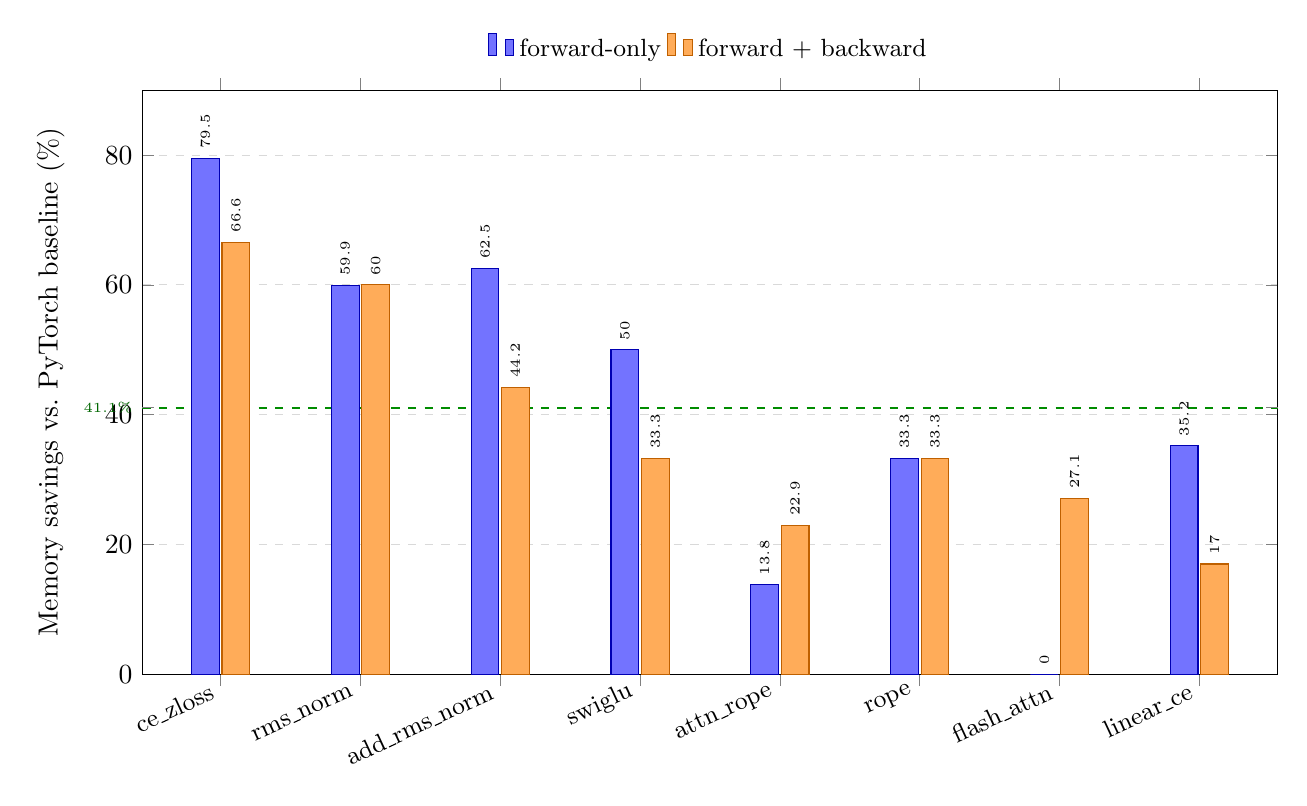
\begin{tikzpicture}
\begin{axis}[
    ybar=1pt,
    bar width=10pt,
    width=16cm,
    height=9cm,
    ymin=0,
    ymax=90,
    ylabel={Memory savings vs.\ PyTorch baseline (\%)},
    symbolic x coords={
        ce\_zloss,
        rms\_norm,
        add\_rms\_norm,
        swiglu,
        attn\_rope,
        rope,
        flash\_attn,
        linear\_ce
    },
    xtick=data,
    x tick label style={rotate=25, anchor=east, font=\small},
    enlarge x limits=0.08,
    legend style={
        at={(0.5,1.03)},
        anchor=south,
        legend columns=2,
        font=\small,
        draw=none
    },
    ymajorgrids=true,
    grid style={dashed, gray!30},
    % 41.1% 均值参考线 (7 个生效算子 fwd+bwd 平均)
    extra y ticks={41.1},
    extra y tick labels={41.1\%},
    extra y tick style={
        grid=major,
        grid style={dashed, green!55!black, line width=0.7pt},
        tick label style={green!40!black, font=\tiny}
    },
    nodes near coords,
    every node near coord/.append style={
        font=\tiny,
        rotate=90,
        anchor=west,
        /pgf/number format/.cd, fixed, precision=1
    },
]

% forward-only memory savings (蓝色) — 数据来自 profile_v2_h800.md
\addplot[fill=blue!55, draw=blue!70!black] coordinates {
    (ce\_zloss,      79.5)
    (rms\_norm,      59.9)
    (add\_rms\_norm, 62.5)
    (swiglu,         50.0)
    (attn\_rope,     13.8)
    (rope,           33.3)
    (flash\_attn,     0.0)
    (linear\_ce,     35.2)
};
\addlegendentry{forward-only}

% forward + backward memory savings (橙色) — 数据来自 profile_bwd_h800.md
\addplot[fill=orange!65, draw=orange!75!black] coordinates {
    (ce\_zloss,      66.6)
    (rms\_norm,      60.0)
    (add\_rms\_norm, 44.2)
    (swiglu,         33.3)
    (attn\_rope,     22.9)
    (rope,           33.3)
    (flash\_attn,    27.1)
    (linear\_ce,     17.0)
};
\addlegendentry{forward + backward}

\end{axis}
\end{tikzpicture}
\end{document}
